\documentclass{article}

% \usepackage[margin=0.5in]{geometry}
\usepackage{arxiv}

\usepackage[utf8]{inputenc} % allow utf-8 input

\usepackage[T1]{fontenc}    % use 8-bit T1 fonts
\usepackage{hyperref}       % hyperlinks
\usepackage{url}            % simple URL typesetting
\usepackage{booktabs}       % professional-quality tables
\usepackage{amsfonts}       % blackboard math symbols
\usepackage{enumitem}
% \usepackage{nicefrac}       % compact symbols for 1/2, etc.
% \usepackage{microtype}      % microtypography
% \usepackage{lipsum}
\usepackage{multicol}
\usepackage{graphicx}
\usepackage{float}
\usepackage{subcaption}
\usepackage[ruled,vlined]{algorithm2e}
% \voffset=-0.5in
% \voffset=0.5in
% \addtolength{\oddsidemargin}{-.875in}
% \addtolength{\evensidemargin}{-.875in}
% \usepackage{indentfirst}
% \usepackage{multirow}

\newcommand{\xsi}{x^{(i)}}
\newcommand{\ysi}{y^{(i)}}

\title{Motion-Based Handwriting Recognition and Word Reconstruction }

% \vspace{-30pt}
\author{
  Junshen Kevin Chen \\
  Stanford University\\
  \texttt{jkc1@stanford.edu} \\
  %% examples of more authors
   \And
  Wanze Xie \\
  Stanford University\\
  \texttt{wanzexie@stanford.edu} \\
    \And
  Yutong He \\
  Stanford University\\
  \texttt{kellyyhe@stanford.edu} \\
}

\begin{document}
% \vspace{-30pt}
\maketitle

% \begin{abstract}
% This is the milestone report for our final project. In the work so far, we have formalized data collection methodology and collected a small sample of preliminary data. This report also discusses some of the key strategies in organizing and processing data for our training work. Then, a preliminary K-means and a K-Medoids model is introduced as a baseline. Finally, this report discusses some of the potential future plans.
% \end{abstract}


\begin{multicols*}{2}

% ============================== begin content ==============================
\vspace{-15px}
\section{Introduction}

Handwriting recognition with vision-based approaches like Optical Character Recognition (OCR) and on-screen stroke-detection has been successful in many applications \cite{bib1, bib2, bib3}. However, such applications or device often require touch screens or digitizers, which are often expensive and pose an unnecessary restriction to the user. Similar challenges are also identified in VR and AR environments \cite{bib4} when user needs to recognize texts with motion sensors without a sensing screen. 

Previously \cite{ours}, we have implemented a handwriting recognition system based on a simple LSTM-based model \cite{lstm} with denoising auto-encoder with decent performance for per-character recognition based solely on the sequential data of pen's rotation during writing. In this project we plan to present extensions to the original system that enhances individual character classification capability and enable handwritten word reconstruction.

Our codes and datasets are available on Github: \url{https://github.com/RussellXie7/cs230\_Final}.

% \begin{figure}[ht]
%     \centering
%     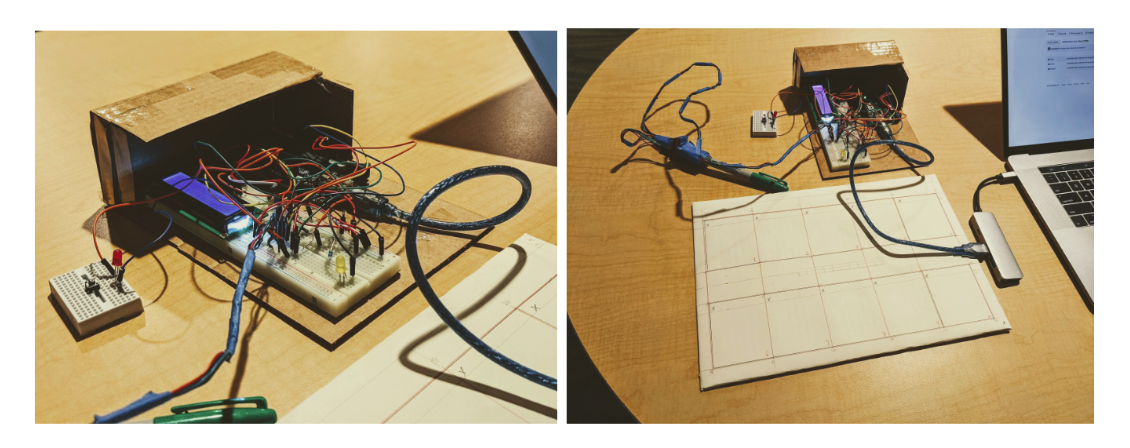
\includegraphics[scale=0.3]{hardware.png}
%     \caption{The hardware we used for data collecting and handwriting recognition}
%     \label{fig:viz_a}
% \end{figure}

\section{Dataset}

\paragraph{Overview and Features} We continue to use a dataset of handwriting sequences of individually written English letters. As in \cite{ours}, a \textbf{sequence} in our setting is defined as the handwriting data for one letter. We have a dataset consisting of sequences from 20 subjects, we ask each subject write each letter 20 times, to a total of 10,400 total sequences. In each sequence, the hardware samples acceleration and rotation each frame, at a variable sampling rate. 

% From the start of subject pressing down the record button, move the stylus to write one single letter, to the release of the button constitutes a \textbf{writing event}, producing data known as a \textbf{sequence}, consisting of as many rows (one row per frame) as the sequence takes.

% \vspace{-5px}
\begin{table}[H]
\centering
\begin{tabular}{lllllll}
\hline
td & yaw    & pitch  & roll   & ax     & ay      & az      \\ \hline
7  & 90.10 & -10.34 & -20.02 & 206.9 & -374.1 & 1052.9 \\
25 & 90.27  & -9.86  & -20.29 & 193.0 & -401.7 & 1046.2 \\ \hline
\end{tabular}
\vspace{3pt}
\caption{Frames from a sample of writing sequence}
\label{tab:sample-sequence}
\end{table}
\vspace{-10px}

\paragraph{Data Augmentation}
Due to the difficulty to collect a large amount of data within the time scope of this project, we implement a data augmentation pipeline to generate new samples by:
\begin{enumerate}
    \item Add a Gaussian noise centered at 0 and with customized small variance (we use 1 in our experiments) to each entry;
    \item Rotate the object by a small random quaternion vector  within $5$ degrees;
    \item Stretch each sequence by three random scalar $\in [1, 1.3]$ constants corresponding to yaw, pitch, roll.
\end{enumerate}

The purpose of data augmentation is to simulate the writing of people with various ways of hand movements. An example of the data augmentation result is as visualized below:

\begin{figure}[H]
    % \raggedleft
    \centering
    \begin{subfigure}[]{0.25\textwidth}
        \centering
        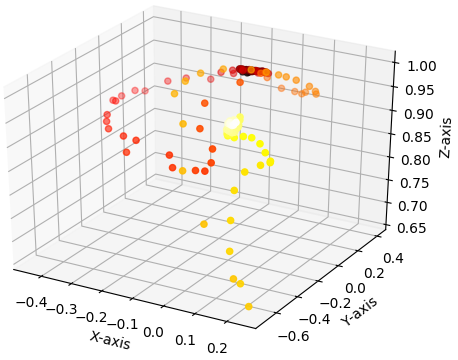
\includegraphics[scale = 0.35 ]{Still_a_5.png}
        \caption{A data sequence for letter "a" without augmentation.}
    \end{subfigure}%
    ~
    \begin{subfigure}[]{0.25\textwidth}
        \centering
        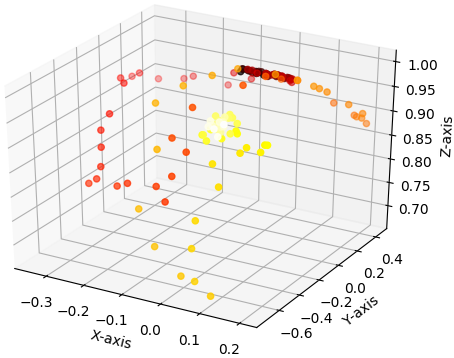
\includegraphics[scale = 0.35]{Still_a_5_aug.png}
        \caption{A data sequence for letter "a" with augmentation.}
    \end{subfigure}
    \caption{Data Augmentation Demonstration}
\end{figure}


\paragraph{Calibration and Normalization} 
The sensor is not by default calibrated before each subject begin writing sequences. Therefore, we ask each subject to hold the stylus upright for 10 seconds, and use the mean of that sensor recording to subtract from all frames recorded from this subject. For rotation values, we want data to be invariant to different subjects' holding the stylus differently, and therefore we also subtract frame 0 of each sequence from all frames in this sequence, to get a delta rotation value.

\paragraph{Test set for word reconstruction} 
A key part of this project is to leverage the classification model for written characters to re-construct the written word, so we need a set of written words as the test set in order to simulate the writing scenario in real time. The structure of frames and sequence is same as the above, however, a sequence now contains one written word instead of single letter. We have collected 40 selected words, each word written 3 times, to a total 360 sequences, to evaluate the model. We expect to collect data from more people in the next step.

\paragraph{Dataset for auto-correct model} 
One of the structures in our word reconstruction system is an auto-correct model to correct the mis-spelled words from a beam search algorithm, due to the potential error from the per-letter classification model. The details to generate training samples for this model is described in Section 4.2, but the raw word corpus we use will be from NLTK \cite{nltk}.

\section{Method}

Our pipeline consists of three components: \textbf{individual character recognition, candidate trajectory generation, and word reconstruction}.

\subsection{Individual Character Recognition}
In our recent work \cite{ours}, we have experimented with different methods ranging from traditional machine learning algorithms such as K Nearest Neighbors\cite{knn}, K Means\cite{kmeans}, and deep learning frameworks such as vanilla CNN\cite{lenet} and LSTM\cite{lstm} with cross entropy loss. Among all the models we have tried, LSTM achieves the best results. Therefore, in this project, we further experiment with RNN models using better model architectures and optimization strategies to improve the accuracy of the individual character recognition task.

Currently, we have made two changes to our model architecture: using a Bidirectional LSTM and adding a dropout layer before the final fully connected layer. The reasoning behind such modification is that our model aims to perform a classification task with access to the entire input data sequence. Even with the autogressive nature of the hand writing sequences, previous research\cite{bilstm} has proven that the ability of accessing both direction of the sequence is beneficial for learning more representative features. Moreover, our model suffered from heavy overfitting the small dataset. By adding the dropout layer, the model should be able to be more generalized than the previous version.

We have experimented with the above modifications and found that adding the right-to-left direction in LSTM does not improve performance. We hypothesize that it is due to the fact that out unidirectional model is able to overfit to the dataset. As a result, additional expressiveness is unnecessary. On the contrary, the dropout layer is able to improve the subject split accuracy from $51\%$ to $54.1\%$by without the autoencoder. Based on the preliminary results, we are going to include a unidirectional LSTM with tuned dropout layers in our final pipeline.

\subsection{Trajectory Search}

To leverage the existing character classfication model to produce a reconstructed word from a continuously written word sequence, we must first slice this sequence into segments, then use the character model to produce logit (and thus probability) to these segments, then search through all possible combinations of these segments to find an optimal trajectories. 

First we define some terminology. As an example, we split a continuously written sequence in to 5 equal parts, this number of granularity is a hyperparameter to be tuned:

\begin{itemize}[leftmargin=*]
    \item \textbf{Bound}: bounds separate a sequence into segments; for this example, the sequence is separated into 5 equal parts, the bounds are indices \texttt{[0,1,2,3,4,5]}
    \item \textbf{Segment}: a segment is a non-empty part of a sequence that are defined by a tuple of its starting and ending bounds; in this example, some segments are \texttt{(0,1), (1,3), (0,4), (0,5)}.
    \item \textbf{Candidate}: a candidate is defined as a four-tuple \texttt{(bound-begin, bound-end, predicted-char, probability)}; each segment produces 26 possible candidates.
    \item \textbf{Trajectory}: a trajectory is a possible way to slice a sequence into several candidates, each candidate corresponding to one predicted character, and thus the trajectory represents one possible prediction of word; a trajectory must span the entire sequence; in this example, a possible trajectory is \texttt{[(0,1,'c',0.9), (1,3,'a',0.8), (3,5,'t',0.85)]}.
\end{itemize}

We define a DP algorithm that searches the all trajectories starting at any arbitrary bound $N$, and ends at $\max(bound)$, then only keeping best $K$ trajectories ("beams") in memory for future search.

\begin{algorithm}[H]
\SetAlgoLined
\caption{PartialTrajectorySearch}
\SetKwInOut{Input}{Input}\SetKwInOut{Output}{Output} 
\Input{$T$, a set of all optimal $K$ trajectories, starting at $N+1$ and ending at $len(S)$}
\Input{$M$, character classification model}
\Input{$K$, number of optimal trajectories to keep}
\Input{$N$, starting point of trajectories towards $len(S)$}
\Input{$S$, written sequence, split into equal parts}

$candidates \gets []$

\For{$N' \gets [N+1, N+2, ..., len(S)]$}{
    $segment \gets S[N:N']$ \\
    $probs \gets \log \left( Softmax(M.forward(segment)) \right)$ \\
    
    \For{$pred \gets [0,1,2,... len(probs)]$ }{
        $prob \gets probs[pred]$ \\
        $C \gets (N, N', pred, prob)$
        
        \For{$T_{future} \in T_{N'}$}{
            $T_{combined} \gets C \cup T_{future}$ \\
            $prob_{combined} \gets AvgProb(T_{combined})$ \\
            $candidates \gets candidates \cup (prob_{combined}, T_{combined})$
        }    
    }
}

$T_N \gets TopK(candidates, K)$\\
yield $T$
\end{algorithm}

The above algorithm has runtime $O(m^2 k)$, where $m$ is the distance between $N$ and end of sequence, $f$ is the complexity of the model to forward propagate one segment. To improve runtime, we may split the sequence into all possible segment, then use the model to forward as a batch, since it is parallelizable. 

Since $PartialTrajectorySearch$ depends on the fact that $\forall N' > N, T_{N'} $ are trajectories already populated, to search for a trajectory optimal to the entire sequence, we will conduct the search starting from the end of the sequence.

\begin{algorithm}[H]
\SetAlgoLined
\caption{TrajectorySearch}
\SetKwInOut{Input}{Input}\SetKwInOut{Output}{Output} 
\Input{$M$, character classification model}
\Input{$K$, number of optimal trajectories to keep}
\Input{$S$, written sequence, split into equal parts}

$T \gets \{\}$

\For{$N \gets [len(s), ..., 2,1,0]$}{
    $PartialTrajectorySearch(T,M,K,N,S)$
}

yield $T_0$
\end{algorithm}

As such, $TrajectorySearch$ yields the globally optimal $K$ trajectories starting at $0$ and spanning the entire sequence. 

\subsection{Word Reconstruction}

Word reconstruction is performed based on the trajectory search results of the input writing sequences. Here we use a auto-correction model to fix common errors in the character prediction and its resulting errors in candidate generation. The auto-correction model details will be described in the next section.

\begin{algorithm}[H]
\SetAlgoLined
\caption{Word reconstruction}
\SetKwInOut{Input}{Input}\SetKwInOut{Output}{Output} \SetKwInOut{Hyperparam}{Hyperparam} 
\Input{$X$, raw written word sequence}
\Input{$M$, character classification model}
\Output{$\hat{y}$, reconstructed word string}
\Hyperparam{$N$, number of segments to split the raw sequence}
\Hyperparam{$K$, number of top trajectories to consider}

$S \leftarrow Split(X, N)$

$\hat{y}s, confidence \leftarrow AutoCorrect (TrajectorySearch(M, K,S))$

yield $\arg \max_{\hat{y} \in \hat{y}s} confidence$

\end{algorithm}

\section{Next Steps}

% [TODO 1]: Confusion Matrix of per-letter accuracy.
% [TODO 2]: New loss function for fine-tune RNN: J(P(A),P(P)) - J(P(A),P(N)) + alpha <= 0.
\subsection{Further Improvement on Individual Character Recognition Model}

\paragraph{Fine-tuning with Common Mistakes and Triplet Loss}
Triplet loss \cite{triplet, triplet2} is a loss function often used for learning similarity problem which can be defined as the following:
$$\mathcal{L} = \max(||f(A) - f(P)||^2-||f(A) - f(N)||^2 + \alpha, 0)$$

where $A$ is the anchor input, $P$ is a positive input, and $N$ is a negative input. $f$ is the usually the embedding function of the input data and $\alpha$ is a hyperparameter that defines the margin between the positive and negative examples.

Here we would like to use the triplet loss with a positive example as another sequence of the same character and a negative example as a sequence of a character that is often confused with the target character, to learn the dissimilarity between different characters and the similarity between the same character written by different subject at different time. We anticipate that fine-tuning the current trained model with triplet loss can enhance the performance of our individual character recognition model.

\paragraph{Attention Mechanism} Adding attention mechanism to the current unidirectional LSTM is another option we have to improve the model performance. The attention mechanism will learn an extra set of weights in parallel to the LSTM cells, which is able to set the important part of the sequence from the unimportant part when rolling through the sequence.

\subsection{Spelling Auto-correction Model}
As in section 3.3, $TrajectorySearch$ algorithm does not guarantee to output the correct word. We then propose to design a Spelling Correction model that attempts to further improve the prediction without improving per-letter recognition accuracy. We plan to explore the two following models:

\paragraph{Baseline Model} Our baseline model will be based on a tool named SymSpell, which is proven \cite{SymSpell} to be effective for correcting misspelled word. With Symmetric Delete spelling correction algorithm, SymSpell can perform edit generation and dictionary lookup for a given Damerau-Levenshtein (DL) distance very fast. This methods does not require training and we decided to apply it for single word spelling correction task.

\paragraph{Deep Learning Based Model} The goal of this model is to improve per-letter prediction from our classification model. In order to generate labeled training samples, we plan to leverage the NLTK word corpus \cite{nltk}. For each letter in a word, we randomly pick a writing sequence of the corresponding letter from the test set, and feed it into our classification model to get a prediction, which may contain mis-predicted letter. The result is then paired with the corresponding word to form one sample of training data and label. 

A recent research \cite{Zhang2019InvestigationOT} in Audio-Speech Recognition (ASR) shows that Transformer can be suitable for spelling correction. Although Transformer is frequently used for sentence related task, we hope to explore its capability for the spelling correction task. Since our setting is intrinsically similar to the ASR problem setting, we believe the spelling correction model should be transferable to our task as well.

% The problem setup for our spell auto-correction model is similar to  Loss function is the sum of the binary cross-entropy of each letter in the word pair across the entire corpus. The evaluation metric will be the accuracy of the model to see if it can calibrate the output from the classification model 


\subsection{Siamese Network - One Shot learning for quick domain adaptation}
If time permits, our last goal is to explore the Siamese architecture \cite{Schroff2015FaceNetAU} to quickly adapt our model to different user's writing habits. The learning strategy is to find a representation in an invariant feature space for a writing sequence through a CNN. As a result, if user provides an example of their handwriting letter, we can quickly recognize user's future handwriting with their canonical writing representation. This makes our model more robust to out-of-domain input.





% \newpage

\bibliographystyle{unsrt}
% to add references, create a file references.bib and populate it in this format:
% https://www.overleaf.com/learn/latex/Bibliography_management_with_bibtex#The_bibliography_file
\bibliography{reference}

% \begin{thebibliography}{1}
%     \bibitem{bib1} Maximilian Schrapel, Max-Ludwig Stadler, and Michael Rohs. 2018. Pentelligence: Combining Pen Tip Motion and Writing Sounds for Handwritten Digit Recognition. In Proceedings of the 2018 CHI Conference on Human Factors in Computing Systems (CHI '18). ACM, New York, NY, USA, Paper 131, 11 pages. DOI: https://doi.org/10.1145/3173574.3173705
%     \bibitem{bib2} Jacob O. Wobbrock, Brad A. Myers, and John A. Kembel. 2003. EdgeWrite: a stylus-based text entry method designed for high accuracy and stability of motion. In Proceedings of the 16th annual ACM symposium on User interface software and technology (UIST '03). ACM, New York, NY, USA, 61-70. DOI: https://doi.org/10.1145/964696.964703 
%     \bibitem{bib3} “US6839464B2 - Multiple Pen Stroke Character Set and Handwriting Recognition System with Immediate Response.” Google Patents, Google, https://patents.google.com/patent/US6839464B2/en.
%     \bibitem{bib4}  I. Poupyrev, N. Tomokazu, and S. Weghorst. 1998. Virtual Notepad: Handwriting in Immersive VR. In Proceedings of the Virtual Reality Annual International Symposium (VRAIS '98). IEEE Computer Society, Washington, DC, USA, 126-.
%     \bibitem{bib5} “US10067568B2 - Augmented reality writing system and method thereof.” Google Patents, Google, https://patents.google.com/patent/US10067568B2/en
%     \bibitem{bib6} Hamed Habibi Aghdam and Elnaz Jahani Heravi. 2017. Guide to Convolutional Neural Networks: A Practical Application to Traffic-Sign Detection and Classification (1st ed.). Springer Publishing Company, Incorporated.
%     \bibitem{bib7} Sepp Hochreiter and Jürgen Schmidhuber. 1997. Long Short-Term Memory. Neural Comput. 9, 8 (November 1997), 1735-1780. DOI=http://dx.doi.org/10.1162/neco.1997.9.8.1735
%     \bibitem{bib8} Stan Salvador and Philip Chan. 2007. Toward accurate dynamic time warping in linear time and space. Intell. Data Anal. 11, 5 (October 2007), 561-580.
% \end{thebibliography}



\end{multicols*}

\end{document}


